% ------------------------------------------------------------------------
% ------------------------------------------------------------------------
% abnTeX2: Modelo de Trabalho Academico (tese de doutorado, dissertacao de
% mestrado e trabalhos monograficos em geral) em conformidade com
% ABNT NBR 14724:2011: Informacao e documentacao - Trabalhos academicos -
% Apresentacao
% ------------------------------------------------------------------------
% ------------------------------------------------------------------------

\documentclass[
	% -- opções da classe memoir --
	12pt,				% tamanho da fonte
	openright,			% capítulos começam em pág ímpar (insere página vazia caso preciso)
	twoside,			% para impressão em recto e verso. Oposto a oneside
	a4paper,			% tamanho do papel.
	% -- opções da classe abntex2 --
	%chapter=TITLE,		% títulos de capítulos convertidos em letras maiúsculas
	%section=TITLE,		% títulos de seções convertidos em letras maiúsculas
	%subsection=TITLE,	% títulos de subseções convertidos em letras maiúsculas
	%subsubsection=TITLE,% títulos de subsubseções convertidos em letras maiúsculas
	% -- opções do pacote babel --
	english,			% idioma adicional para hifenização
	brazil,				% o último idioma é o principal do documento
	svgnames
	]{abntex2}\usepackage[]{graphicx}\usepackage[]{color}
% maxwidth is the original width if it is less than linewidth
% otherwise use linewidth (to make sure the graphics do not exceed the margin)
\makeatletter
\def\maxwidth{ %
  \ifdim\Gin@nat@width>\linewidth
    \linewidth
  \else
    \Gin@nat@width
  \fi
}
\makeatother

\definecolor{fgcolor}{rgb}{0.345, 0.345, 0.345}
\newcommand{\hlnum}[1]{\textcolor[rgb]{0.686,0.059,0.569}{#1}}%
\newcommand{\hlstr}[1]{\textcolor[rgb]{0.192,0.494,0.8}{#1}}%
\newcommand{\hlcom}[1]{\textcolor[rgb]{0.678,0.584,0.686}{\textit{#1}}}%
\newcommand{\hlopt}[1]{\textcolor[rgb]{0,0,0}{#1}}%
\newcommand{\hlstd}[1]{\textcolor[rgb]{0.345,0.345,0.345}{#1}}%
\newcommand{\hlkwa}[1]{\textcolor[rgb]{0.161,0.373,0.58}{\textbf{#1}}}%
\newcommand{\hlkwb}[1]{\textcolor[rgb]{0.69,0.353,0.396}{#1}}%
\newcommand{\hlkwc}[1]{\textcolor[rgb]{0.333,0.667,0.333}{#1}}%
\newcommand{\hlkwd}[1]{\textcolor[rgb]{0.737,0.353,0.396}{\textbf{#1}}}%
\let\hlipl\hlkwb

\usepackage{framed}
\makeatletter
\newenvironment{kframe}{%
 \def\at@end@of@kframe{}%
 \ifinner\ifhmode%
  \def\at@end@of@kframe{\end{minipage}}%
  \begin{minipage}{\columnwidth}%
 \fi\fi%
 \def\FrameCommand##1{\hskip\@totalleftmargin \hskip-\fboxsep
 \colorbox{shadecolor}{##1}\hskip-\fboxsep
     % There is no \\@totalrightmargin, so:
     \hskip-\linewidth \hskip-\@totalleftmargin \hskip\columnwidth}%
 \MakeFramed {\advance\hsize-\width
   \@totalleftmargin\z@ \linewidth\hsize
   \@setminipage}}%
 {\par\unskip\endMakeFramed%
 \at@end@of@kframe}
\makeatother

\definecolor{shadecolor}{rgb}{.97, .97, .97}
\definecolor{messagecolor}{rgb}{0, 0, 0}
\definecolor{warningcolor}{rgb}{1, 0, 1}
\definecolor{errorcolor}{rgb}{1, 0, 0}
\newenvironment{knitrout}{}{} % an empty environment to be redefined in TeX

\usepackage{alltt}

% ---
% Novo list of (listings) para QUADROS
% ---

\newcommand{\quadroname}{Quadro}
\newcommand{\listofquadrosname}{Lista de quadros}

\newfloat[chapter]{quadro}{loq}{\quadroname}
\newlistof{listofquadros}{loq}{\listofquadrosname}
\newlistentry{quadro}{loq}{0}

% configurações para atender às regras da ABNT
\counterwithout{quadro}{chapter}
\renewcommand{\cftquadroname}{\quadroname\space}
\renewcommand*{\cftquadroaftersnum}{\hfill--\hfill}

% ---
% PACOTES
% ---

% ---
% Pacotes fundamentais
% ---
\usepackage{lmodern}			% Usa a fonte Latin Modern
\usepackage[T1]{fontenc}		% Selecao de codigos de fonte.
\usepackage[utf8]{inputenc}		% Codificacao do documento (conversão automática dos acentos)
\usepackage{indentfirst}		% Indenta o primeiro parágrafo de cada seção.
\usepackage{color}			% Controle das cores
\usepackage{graphicx}			% Inclusão de gráficos
\usepackage{microtype} 			% para melhorias de justificação
\usepackage{setspace}
\usepackage{wrapfig}

% ---
% Para titulo em destaque sem sequencia de numeração
% ---
\newcommand{\datatitle}[1]{
  \normalsize \textsc{#1}
}

% ---
% Funções matematicas
% ---
\usepackage{amsmath,amssymb,amstext}
\usepackage{mathtools}                  % Funcionalidades (como \dcases)
\usepackage{dsfont}    %% Para \mathds{1} Indicadora
\usepackage{bm}

\DeclareMathOperator{\Ell}{\mathcal{L}}
\DeclareMathOperator{\R}{\mathbb{R}}
\DeclareMathOperator{\ind}{\mathds{1}}

\DeclareRobustCommand{\rchi}{{\mathpalette\irchi\relax}}
\newcommand{\irchi}[2]{\raisebox{\depth}{$#1\chi$}}

% ---
% Para tabelas
% ---
\usepackage{multirow}
\usepackage{array}
\usepackage{threeparttable}

% ---
% Pacotes e definições adcionais, para adequações especificas
% ---
\usepackage{tikz}
\usepackage{pdflscape}			% para ambiente landscape
\usepackage{pgfgantt}			% cronograma estilo gráfico de gantt
\usepackage{multicol}
\usetikzlibrary{backgrounds}
\usepackage{tasks}

% ---
% Fontes matemáticas
% ---
\usepackage{mathpazo}
\usepackage{inconsolata}
\usepackage{verbatim}

% ---
% Pacotes adicionais, usados apenas no âmbito do Modelo Canônico do abnteX2
% ---
\usepackage{lipsum}				% para geração de dummy text
% ---

% ---
% Pacotes de citações
% ---
\usepackage[brazilian,hyperpageref]{backref}% Paginas com as citações
\usepackage[alf, abnt-etal-list=0]{abntex2cite}				% Citações padrão ABNT

% ---
% CONFIGURAÇÕES DE PACOTES
% ---

% ---
% Configurações do pacote backref
% Usado sem a opção hyperpageref de backref
\renewcommand{\backrefpagesname}{Citado na(s) página(s):~}
% Texto padrão antes do número das páginas
\renewcommand{\backref}{}
% Define os textos da citação
\renewcommand*{\backrefalt}[4]{
  \ifcase #1 %
  Nenhuma citação no texto.%
  \or
  Citado na página #2.%
  \else
  Citado #1 vezes nas páginas #2.%
  \fi}%
% ---

% ---
% Informações de dados para CAPA e FOLHA DE ROSTO
% ---
\titulo{Resenhas da disciplina Seminários PPGInf}
\vspace{2cm}
\autor{Lineu Alberto Cavazani de Freitas}
\local{Curitiba}
\data{2020}
\instituicao{Universidade Federal do Paraná
  \par
  Setor de Ciências Exatas
  \par
  Programa de Pós graduação em Informática
}
\orientador[Professor:]{Dr. Luis Carlos Erpen Bona}
\tipotrabalho{Avaliação}
% O preambulo deve conter o tipo do trabalho, o objetivo,
% o nome da instituição e a área de concentração
\preambulo{Trabalho apresentado à disciplina
    de seminários do Programa de Pós Graduação em Informática da Universidade
    Federal do Paraná.}
% ---

% ---
% Configurações de aparência do PDF final

% informações do PDF
\makeatletter
\hypersetup{
  % pagebackref=true,
  pdftitle={\@title},
  pdfauthor={\@author},
  pdfsubject={\imprimirpreambulo},
  pdfcreator={LaTeX with abnTeX2},
  % pdfkeywords={abnt}{latex}{abntex}{abntex2}{projeto de pesquisa},
  colorlinks=true,	% false: boxed links; true: colored links
  linkcolor=blue,     % color of internal links
  citecolor=blue, % color of links to bibliography
  filecolor=magenta, % color of file links
  urlcolor=black,
  bookmarksdepth=4
}
%\addto\captionsbrazil{
%  \renewcommand{\bibname}{REFER\^ENCIAS}
%}
%\makeatother
% ---

% ---
% Espaçamentos entre linhas e parágrafos
% ---

% O tamanho do parágrafo é dado por:
\setlength{\parindent}{1.3cm}

% Controle do espaçamento entre um parágrafo e outro:
\setlength{\parskip}{0.2cm}  % tente também \onelineskip

% ---
% Highlight knitr code (pode-usar usar os varios highligths já definidos
% com thm = knit_theme$get("nuvola"); knit_theme$set(thm))
% ---

\renewcommand{\hlnum}[1]{\textcolor[rgb]{0.733,0,1}{#1}}%
\renewcommand{\hlstr}[1]{\textcolor[rgb]{0,0.533,0}{#1}}%
\renewcommand{\hlcom}[1]{\textcolor[rgb]{0,0,0}{#1}}%
\renewcommand{\hlopt}[1]{\textcolor[rgb]{0.412,0.412,0.412}{#1}}%
\renewcommand{\hlstd}[1]{\textcolor[rgb]{0.2,0.2,0.2}{{#1}}}%
\renewcommand{\hlkwa}[1]{\textcolor[rgb]{0.2,0.2,0.2}{{#1}}}%
\renewcommand{\hlkwb}[1]{\textcolor[rgb]{0.4,0,0}{\textbf{#1}}}%
\renewcommand{\hlkwc}[1]{\textcolor[rgb]{0.13,0.29,0.53}{#1}}%
\renewcommand{\hlkwd}[1]{\textcolor[rgb]{0.13,0.29,0.53}{\textbf{#1}}}%

% ---
% compila o indice
% ---
\makeindex
% ---

% ----
% Início do documento
% ----
\IfFileExists{upquote.sty}{\usepackage{upquote}}{}
\begin{document}

% Seleciona o idioma do documento (conforme pacotes do babel)
% \selectlanguage{english}
\selectlanguage{brazil}

% Retira espaço extra obsoleto entre as frases.
\frenchspacing

% ----------------------------------------------------------
% ELEMENTOS PRÉ-TEXTUAIS
% ----------------------------------------------------------
% \pretextual

% ---
% Capa
% ---
\tikz[remember picture,overlay] \node[opacity=1,inner sep=0pt] at
(current page.center){
  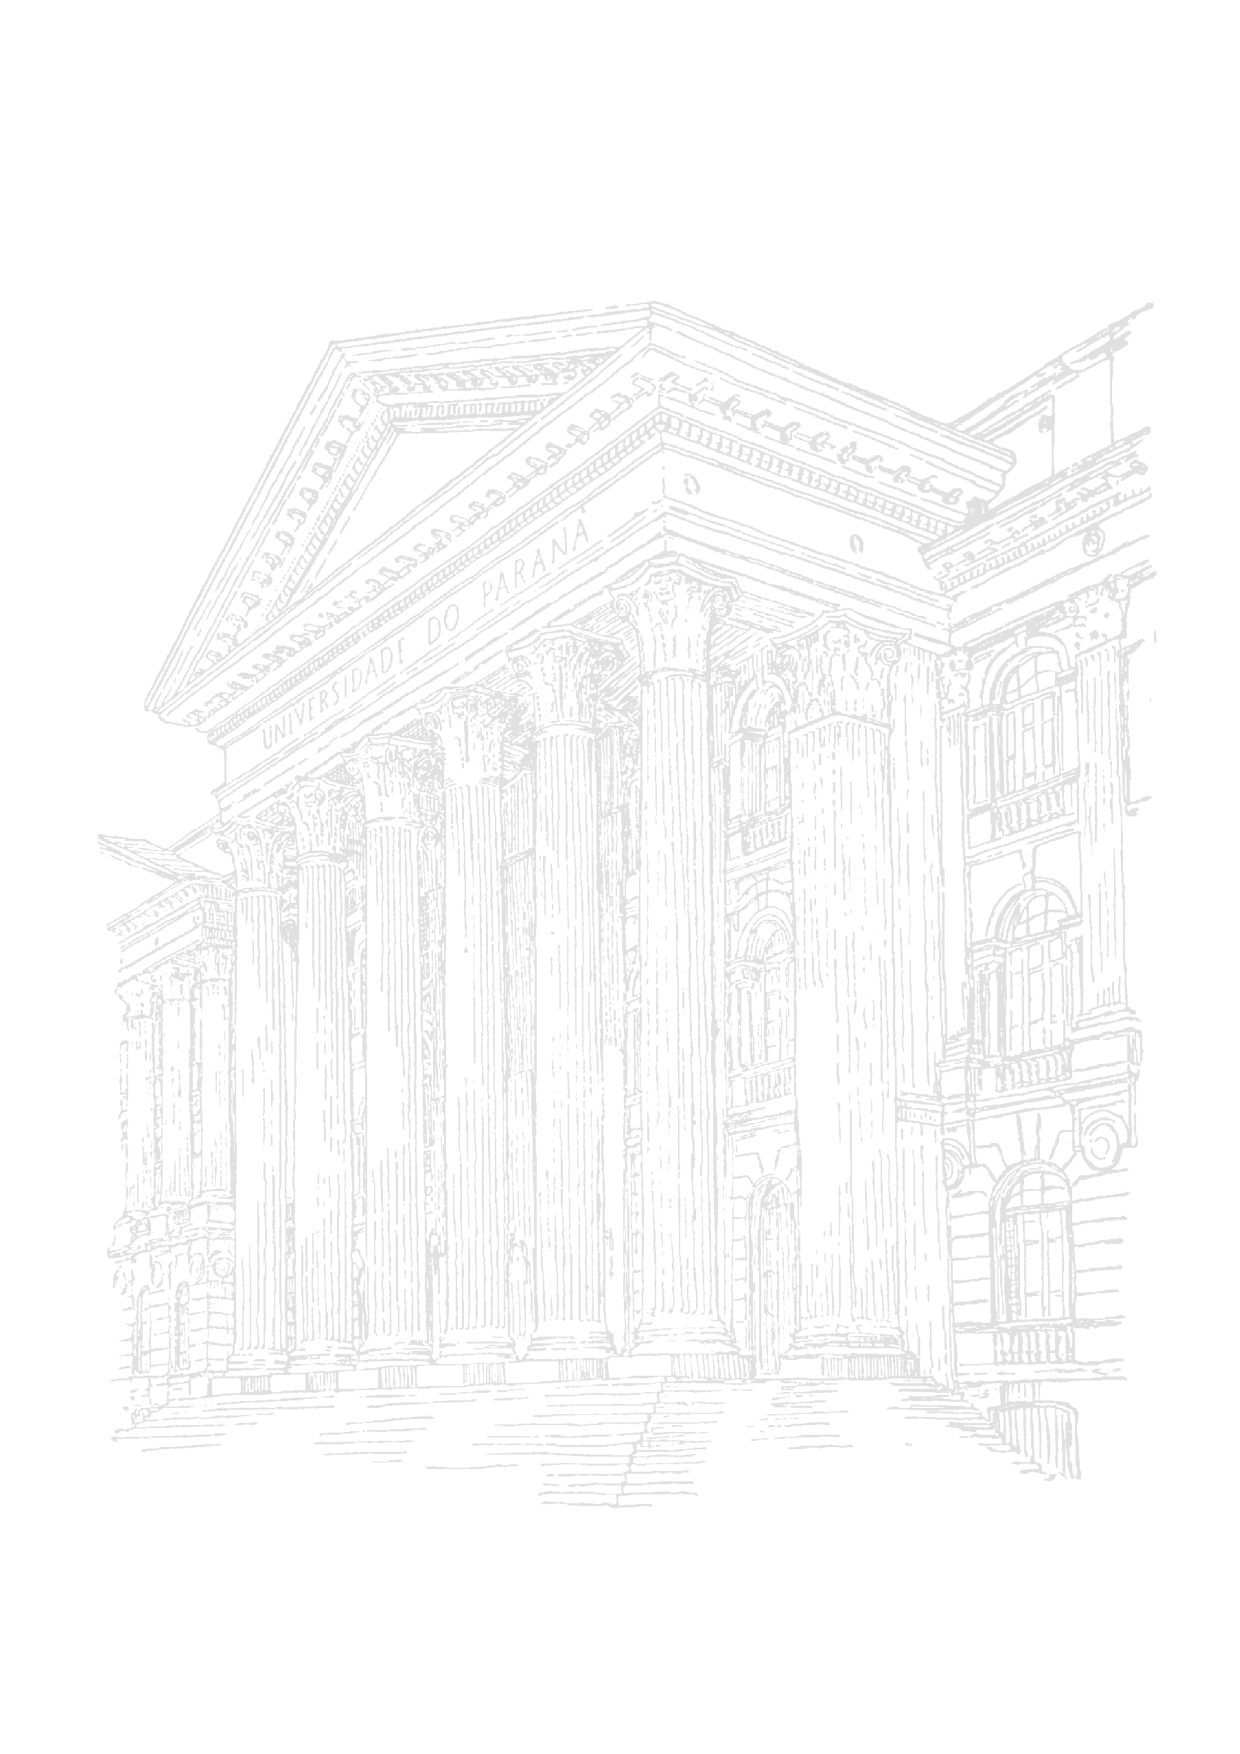
\includegraphics[width=\paperwidth,
  height=\paperheight]{images/ufpr_bg}};

\begin{center}
  {\Large \textsf{Universidade Federal do Paraná}}
  \vspace{-0.5cm}
\end{center}

\imprimircapa

% ---

% ---
% Folha de rosto
% ---
\imprimirfolhaderosto
% ---

% ---
% Dedicatória
% ---
% \begin{dedicatoria}
%   \lipsum[1]
% \end{dedicatoria}
% ---

% ---
% Agradecimentos
% ---
% \begin{agradecimentos}
%   \lipsum[1]
% \end{agradecimentos}
% ---

% ---
% Epígrafe
% ---
%\begin{epigrafe}
%    \vspace*{\fill}
%	\begin{flushright}
%          \textit{``Software is like sex: it's better when \\
%            it's free``}\\
%          --- Linus Torvalds \\[1cm]

%          \textit{``The numbers are where the scientific \\ discussion
%            should start, not end.''}\\
%          --- Steven N. Goodman
%	\end{flushright}
%\end{epigrafe}
% ---

% ---
% RESUMOS
% ---

% resumo em português
% \setlength{\absparsep}{18pt} % ajusta o espaçamento dos parágrafos do resumo
% \begin{resumo}
% 
% Seminários sobre o estado da arte em diversas especialidades da Ciência da Computação. Seminários assistidos:
% 
% \begin{itemize}
%   
%   \item 25 de maio, COVID-19 – Conceitos de epidemiologia, Bernardo Montesanti Machado de Almeida, Medico infectologista da Unidade de Vigilancia em Saúde do CHC/UFPR.
%   
%   \item
%   
% \end{itemize}
% 
% \end{resumo}

% ---
% inserir lista de ilustrações
% ---
%\pdfbookmark[0]{\listfigurename}{lof}
%\listoffigures*
%\cleardoublepage
% ---

% ---
% inserir lista de tabelas
% ---
%\pdfbookmark[0]{\listtablename}{lot}
%\listoftables*
%\cleardoublepage
% ---

% ---
% inserir lista de quadros
% ---
%\pdfbookmark[0]{\listofquadrosname}{loq}
%\listofquadros*
%\cleardoublepage
% ---

% ---
% inserir lista de abreviaturas e siglas
% ---
% \begin{siglas}
%   \item[ABNT] Associação Brasileira de Normas Técnicas
%   \item[abnTeX] ABsurdas Normas para TeX
% \end{siglas}
% ---

% ---
% inserir lista de símbolos
% ---
% \begin{simbolos}
%   \item[$ \log $] Logarítmo neperiano (de base $e$).
%   \item[$ \ell $] log-verossimilhança maximizada.
%   \item[AIC] Critério de Informação de Akaike, do inglês \textit{Akaike
%       Information Criterion}.
% \end{simbolos}
% ---

% ---
% inserir o sumario
% ---
\pdfbookmark[0]{\contentsname}{toc}
\tableofcontents*
\cleardoublepage
% ---

% ----------------------------------------------------------
% ELEMENTOS TEXTUAIS
% ----------------------------------------------------------
\textual

\chapter{COVID-19 – Conceitos de epidemiologia}
\label{cap:res1}

% ----------------------------------------------------------------------
% COVID-19 – Conceitos de epidemiologia
% ----------------------------------------------------------------------

Resenha do seminário ministrado no dia 25/05/2020 no Programa de Pós Graduação em Informática da UFPR por Bernardo Montesanti Machado de Almeida(médico infectologista da Unidade de Vigilância em Saúde do CHC/UFPR) e Wagner Hugo Bonat (professor do Departamento de Estatística da UFPR).

No seminário foi apresentado o conceito de taxa de reprodução, denotada por $R_t$ que estima a disseminação de uma doença infectocontagiosa. Trata-se do número esperado de transmissões que devem ocorrer a partir de um caso. Dito isso, existem 3 possíveis resultados: $R_t = 1$, isto é, um infectado transmite para apenas uma pessoa, representa o cenário de equilíbrio endêmico. $R_t < 1$, trata-se da chamada supressão endêmica. E, por fim, $R_t > 1$ representa o cenário de ciclo epidêmico, no qual um infectado transmite para mais de um indivíduo o que gera a tão falada curva exponencial de casos. O ideal é atingir o cenário de supressão pois este indica queda progressiva na incidência considerando que sejam mantidas as condições daquele momento.

Contudo vale ressaltar que os valores de $R$ são sensíveis à dinâmica da doença e a fatores como localidade e clima. Como exemplo de ilustração, o doutor Bernardo citou o impacto do fator climático na pandemia de H1N1, em 2009, que fez com que a taxa de reprodução fosse superior a 2 no Paraná enquanto que a taxa era consideravelmente menor no restante dos estados brasileiros com clima mais quente.



Na atual pandemia do novo coronavírus, a taxa de reprodução varia entre 2 e 3, e é consideravelmente mais alta do que outras pandemias históricas como H1N1, Ebola e gripe espanhola.



Tratando mais a respeito do Corona vírus: a COVID-19 é uma doença causada pelo coronavírus SARS-CoV-2, descoberto em 31/12/19 após casos registrados na China. De acordo com a Organização Mundial de Saúde (OMS), cerca de 80\% dos infectados podem ser assintomáticos e cerca de 20\% podem requerer atendimento hospitalar por apresentarem dificuldade respiratória. 



Os sintomas da COVID-19 podem variar de um simples resfriado até uma pneumonia severa. A transmissão acontece por meio de toque (na pessoa ou em superfície contaminada), gotículas de saliva, espirro, tosse, catarro, etc. O diagnóstico é feito através de exames laboratoriais.
Na prática, trata-se de um vírus com letalidade baixa mas altamente contagioso e que, até o momento, não há vacina. Portanto, caso a disseminação não seja devidamente controlada, é uma doença capaz de levar sistemas de saúde inteiros ao colapso como ocorreu em diversos países do mundo. Todavia, devido à variedade de sintomas, controlar a cadeia de transmissão se torna uma tarefa difícil considerando que boa parte dos casos são assintomáticos, diferente de doenças conhecidas como Ebola, por exemplo, em que os sintomas são tão mais violentos que se torna uma tarefa fácil identificar o indivíduo contaminado e isolá-lo, acabando com a cadeia de transmissão que seria gerada por esse indivíduo.



Por esta razão justifica-se a estratégia de distanciamento social para conter a disseminação da doença, pela dificuldade de isolar apenas aqueles infectados dado que muitos casos são silenciosos e a taxa de reprodução é alta.



Por mais que em termos percentuais não seja uma doença com alto índice de casos graves e letalidade, a taxa de reprodução é a maior preocupação pois 20\% de um número altíssimo de contaminados que terão sintomas graves, necessitarão de atendimento intensivo congestionando o sistema de saúde de tal forma que não haja leitos o suficiente para lidar com os casos graves de coronavírus e também para casos de outras doenças e circunstâncias que levem o indivíduo a necessitar de terapia intensiva; deste modo fazendo que a letalidade de todas as doenças que necessitam terapia intensiva aumente, e não apenas dos casos de COVID-19.



Outro fato que gera preocupação é o efeito que os cenários divulgados causam na população ao observar-se valores de taxas de contágio e resultados de modelos que apontam para o cenário de situação sob controle, pois estes resultados geram um afrouxamento das medidas de isolamento (atualmente nossa única medida protetiva na ausência de uma vacina) e causam a elevação das contaminações. Deste modo cria-se um ciclo vicioso, no qual as análises mostram que a situação dá indícios de estar sob controle, afrouxam-se as medidas restritivas, como resultado do afrouxamento a contaminação aumenta, o que nos obriga a retomar as medidas de isolamento e assim por diante.



Outro assunto que tem sido particularmente tratado é o termo imunidade de rebanho. A ideia consiste em imunizar boa parte da população de modo que os que não foram imunizados estejam protegidos. O problema é que com a ausência de uma vacina, este tipo de imunização se daria pelo contágio (a pessoa contaminada cria anticorpos e não contamina mais, está imune). Assim, imaginemos um cenário hipotético: digamos que para atingir imunidade de rebanho precisaríamos de, sendo otimista, 2/3 da população imunizada. Considerando que a população brasileira atualmente é aproximadamente 210 milhões, necessitaríamos de 138 milhões de pessoas (2/3) contaminadas. Contudo, destas 138 milhões,  por volta de 27 milhões de pessoas necessitariam de atendimento intensivo devido à sintomas graves (20\% dos infectados, como indica a OMS). Atualmente a letalidade no Brasil relacionada ao coronavírus está em torno de 6\%, deste modo, considerando este cenário, haveriam 8 milhões de óbitos. Nota-se que é um cenário completamente inviável.



\chapter{Fortes correlações entre o crescimento (tipo Lei de Potência) da COVID-19 em quatro continentes e a ineficiência das estratégias suaves de quarentena}
\label{cap:res2}

% ----------------------------------------------------------------------
% Fortes correlações entre o crescimento (tipo Lei de Potência) da COVID-19 em quatro continentes e a ineficiência das estratégias suaves de quarentena
% ----------------------------------------------------------------------

Resenha do seminário ministrado no dia 28/05/2020 no Programa de Pós Graduação em Física da UFPR por Marcus Beims (professor do Departamento de Física da UFPR).

No seminário ministrado pelo professor Marcus Beims foi apresentado um breve contexto a respeito de modelos epidemiológicos, como o modelo de suscetíveis e imunes (SI), o modelo de suscetíveis, infectados e recuperados (SIR) e o modelo Suscetíveis, Expostos, Infectados e Recuperados (SEIR).

No trabalho foi utilizado o modelo SEIR para descrever a contaminação e estudar melhores estratégias para atingir o famoso achatamento da curva. Uma das conclusões é que modelos epidemiológicos podem ser descritos por redes de “mundo pequeno” ou “livres de escala”. 

Além disso foram apresentadas técnicas para obtenção de medidas de correlação entre tempo e número de casos acumulados e também do potencial de curvas de crescimento de casos de Covid-19 ajustadas via Lei de Potência ao invés da famosa curva exponencial, amplamente utilizada e atualmente discutida no atual cenário de pandemia.
 
Os resultados mostram que as estratégias de contenção são igualmente válidas em diferentes países o que refuta argumentos muito ditos no cenário atual de que deve-se regionalizar a política de isolamento no Brasil dado seu território.

Outro importante resultado ressalta a importância do isolamento social para contenção do alastramento da doença considerando o potencial de disseminação do vírus e a dificuldade de identificar e isolar infectados durante a fase de contaminação fazendo com que o isolamento seja, no cenário atual, nossa única linha de defesa na ausência de uma vacina.

Segundo o estudo, um distanciamento social mediano, junto com a identificação e isolamento diário de poucos dos indivíduos infectados assintomáticos, não é suficiente para diminuir significativamente o avanço do número de casos. Mostrando que as demandas e desafios atuais são encontrar meios eficientes para se identificar indivíduos contaminados que sejam assintomáticos visando o isolamento destes para que não contaminem demais indivíduos e, enquanto isso não seja possível, aumentar e reforçar de forma significativa as medidas de distanciamento social. 

Deste modo, dadas as circunstâncias e dificuldades no cenário atual, nossa melhor chance para diminuição do número de infectados são implementar eficazes medidas de isolamento social combinadas à realização periódica massiva de testes que viabilizam diagnosticar indivíduos infectados assintomáticos com o objetivo de isolá-los de forma efetiva de tal modo que a taxa de reprodução deste indivíduo seja neutralizada. Deste modo, a longo prazo a taxa de reprodução geral será reduzida e sairemos do risco de colapsar o sistema de saúde. 

\chapter{Overview das pesquisas multidisciplinares do Setor de Exatas em época de pandemia}
\label{cap:res3}

% ----------------------------------------------------------------------
% Overview das pesquisas multidisciplinares do Setor de Exatas em época de pandemia
% ----------------------------------------------------------------------

Resenha do seminário ministrado no dia 29/05/2020 no Programa de Pós Graduação em Informática da UFPR por Marcos Sunye (diretor do setor de ciências exatas da UFPR).

No seminário ministrado pelo professor Marcos Sunye foram apresentadas as diversas iniciativas de cursos, programas de pós graduação, professores e pesquisadores das exatas em estudos e iniciativas com o objetivo de compreender, conter e divulgar informações de forma correta a respeito do novo corona vírus.  O Setor de Ciências Exatas possui 6 departamentos, 7 programas de pós graduação e todos estão envolvidos de algum modo em trabalhos a respeito do Covid-19.

As ações vão desde a produção de álcool em gel feita pelo Departamento de Química, passando pelo uso de impressoras 3D pela Expressão Gráfica para impressão de materiais de segurança até estudos sobre a disseminação da doença e estratégias de contenção e diagnóstico.

Existe a iniciativa Portal Covid-19 que tem por objetivo agregar informações, modelos e visualizações de dados sobre a pandemia. Com contribuições de pesquisadores dos Departamentos de Estatística, Informática, Física, Matemática e Saúde da Universidade.

Além disso existem projetos vinculados à pesquisadores da Física como o do professor Marcus Beims que faz uso do modelo SEIR para entender de que forma se propaga o vírus e sugerir medidas e estratégias para conter sua disseminação.

Há também projetos com foco em testagem, como o do professor David Menotti que faz uso de técnicas de processamento de imagem, visão computacional e aprendizado de máquinas para diagnóstico em que a entrada é uma radiografia do pulmão do paciente.

E diversos outros projetos em andamento que avaliam a viabilidade e como proceder de forma segura e eficiente o retorno das atividades, como de que forma manter a disposição dos laboratórios e técnicas para aferição de temperatura dos alunos que entram nas instalações da Universidade, por exemplo.

\chapter{Mulheres nas Ciências: ações de Pesquisa e Extensão}
\label{cap:res4}

% ----------------------------------------------------------------------
% Mulheres nas Ciências: ações de Pesquisa e Extensão
% ----------------------------------------------------------------------

Resenha do seminário ministrado no dia 01/06/2020 no Programa de Pós Graduação em Informática da UFPR por Camila Silveira da Silva (professora do Departamento de Química da UFPR).

No seminário mistrado pela professora Camila Silveira foram abordados aspectos da evidente desigualdade de gênero nas ciências de modo geral e, mais especificamente, nas ciências exatas, onde a ausência de equidade é ainda mais gritante.

Numa primeira provocação a professora sugeriu que fizéssemos um questionamento: quantas mulheres cientistas você conhce? O que prontamente nos mostra como a imagem de cientista está vinculada à figura esteriotipada de homem branco no laboratório.

Após este exercício foram apresentadas uma série de motivos da necessacidade de se falar sobre mulheres na ciência na atualidade como o fato de apenas 30\% de pesquisadores de ciência e tecnologia serem do sexo feminino, percentual bastante distante de um nível real de representatividade. Além disso, desde 1901 apenas 5\% dos prêmios Nobel foram destinados a pesquisadoras.

Foi discutida também a ausência políticas que busquem igualdade de gênero nas universidades e a falta de incentivo ao sexo feminino para se fazer ciência, o que vem desde a infância com brinquedos temáticos sendo destinados à seção masculina de lojas infantis e vão até os desafios enfrentados por mulheres na academia, como comentários inadequados feitos por colegas homens e maternidade, grande fator de evasão entre as mulheres.

Dentre os 17 objetivos listados pela ONU visando desenvolvimento sustentável até 2030, um deles diz respeito à igualdade de gênero e tem como metas acabar com a desigualdade de gênero, eliminar toda e qualquer forma de violência contra a mulher, garantir a participação de mulheres com igualdade de oportunidade em todas as esferas da sociedade desde recursos econômicos até oportunidade de liderança na vida política, econômica e pública.

Por fim, foram apresentados uma série de movimentos atuais que buscam atingir estes objetivos nacional e internacionalmente com ênfase no Projeto de Extensão da Universidade Federal do Paraná Meninas e Mulheres na Ciência que conta com a participação de professoras e docentes de graduação e pós graduação das mais diversas áreas da Universidade.

\chapter{Software Modernization}
\label{cap:res5}

% ----------------------------------------------------------------------
% Software Modernization
% ----------------------------------------------------------------------

Resenha do seminário ministrado no dia 01/06/2020 no Programa de Pós Graduação em Ciência da Computação da UTFPR por Wesley Klewerton (professor na UTFPR).

O trabalho apresentado pelo professor Wesley Klewerton tinha como objetivo definir e implementar uma metodologia automatizada para re-engenharia de um conjunto de modelos dentro de um Software Product Line Engineering (SPL).

Engenharia de Software área da Computação que se propõe a estudar e propor soluções para desenvolver sistemas de software de forma produtiva. Tarefa que em geral envolve partes complexas como produto (o que será o resultado final), processo (como fazer) e autores (individual, equipe, etc). Além disso, na Engenharia de Software, deve haver uma preocupação com a qualidade interna (aquela que diz respeito aos desenvolvedores) e externa (que diz respeito ao usuário).

Software modernization é uma área de Engenharia de Software que trata de problemas como conversão, reescrita ou portabilidade de sistemas para uma versão mais moderna de linguagem, protocolos ou hardware. Pode se tratar de uma tarefa custosa devido ao risco, dificuldade e à ausência de uma ferramenta de propósito geral para realização desta tarefa (por mais que hajam algumas técnicas específicar para fazê-lo).

A necessidade da modernização pode levar à re-engenharia, migração, substituição e reuso. A reutilização trata-se da reciclagem, isto é, aproveitar um projeto já existente e modificá-lo para obter outro produto final. Existem técnicas como Software Product Line Engineering (SPL) que é um paradigma para sistematização das técnicas de reuso. Já a re-engenharia é a análise e alteração de um sistema a fim de sua reestruturação em uma nova forma e, este trabalho para SPLs consiste de diferentes fases e propósitos. Trata-se de um tema complexo e de literatura limitada e , no trabalho, foi proposta uma implementação de metodologia automatizada para re-engenharia de um conjunto de modelos dentro de um SPL.

\chapter{Ligados pela linguagem: diálogos possíveis entre linguistas e cientistas de computação}
\label{cap:res6}

% ----------------------------------------------------------------------
% Ligados pela linguagem: diálogos possíveis (e necessários) entre linguistas e cientistas de computação
% ----------------------------------------------------------------------

Resenha do seminário ministrado no dia 05/06/2020 no Programa de Pós Graduação em Informática da UFPR por Adelaide H. Pescatori Silva (professora do Departamento de Letras UFPR e pós-doc PPGInf).

No seminário ministrado pela professora Adelaide foram tratados num primeiro momento as similaridades entre linguística (estudo da linguagem humana) e computação (análise de dados através de linguagens artificiais) e a sua relação com um mesmo objeto de interesse: a linguagem. 

Foi apresentado que a linguística é construída por partes ou módulos e a compreensão da estrutura geral e de cada módulo auxilia na compreensão do todo, enquanto que, de modo similar, na programação, apenas alguns pequenos blocos de funcionalidades, quando combinados, são suficientes para solucionar diversos tipos de problema. Outro ponto interessante comentado foi a semelhança entre os diagramas do processamento da fala humana por um falante e o processamento de dados feito por um computador e que, em ambos os casos, há um papel fundamental da memória.

Um ponto histórico em que a convergência entre linguística e computação resultou num produto foi o desenvolvimento de "máquinas falantes" que, dentre as possíveis funcionalidades pode-se citar síntese, tradução e até mesmo a própria comunicação entre humano e máquina. Além de outros produtos gerados ao longo do tempo como ferramentas de tradução automática, reconhecimento e interpretação de fala, classificação e produção de textos, sistemas de busca, etc.

Foi apresentada também a grande similaridade entre o processo de estudos a respeito de linguística e o processo percorrido pela ciência de dados, que consiste em: fazer uma pergunta (hipótese), coletar dados, tratá-los e explorálos, buscar modelos que permitam inferir os resultados amostrais para uma população e por fim, interpretar os resultados de modo a verificar se a hipótese inicial foi ou não aceita, isto é, se há evidência suficiente para rejeitar ou não a hipótese inicialmente levantada.

Por fim a professora Adelaide apresentou o plano do seu trabalho de pós-doc: a criação de um jogo para fixação de normas ortográficas de modo contextualizado em que o público alvo seriam alunos do Fundamental II (6º ao 9º ano) que faz uso de linguística probabilística e técnicas de aprendizado de máquina. Um plano altamente motivado pelo atual cenário de pandemia em que se fazem necessárias ferramentas educacionais remotas.

\chapter{Dançando com robôs: planejamento automático de mitigação intermitente para Covid-19}
\label{cap:res7}

% ----------------------------------------------------------------------
% Dançando com robôs: planejamento automático de mitigação intermitente para Covid-19
% ----------------------------------------------------------------------

Resenha do seminário ministrado no dia 05/06/2020 no Programa de Pós Graduação em Matemática da UFPR por Paulo J.S. Silva (professor do IMECC-Unicamp).

No seminário o professor Paulo foram apresentados estratégias e modelos que visam lidar de forma mais eficiente com questões como isolamento social em tempos de pandemia de tal modo que proteja a população do contágio e sem que a economia seja tão afetada. 

A discussão iniciou-se na contextualização dos protocolos de distanciamento social incialmente aplicados: tratam-se de protocolos que adiam o problema, considerando que não geram imunização da população. Além disso  os protocolos iniciais eram ineficientes por não analisar questões como a infraestrutura de cada regionalidade. No estado de São Paulo foi implantado um novo protocolo que olha para a capacidade de cada local. Deste modo, o objetivo era chegar a um modelo que pudesse organizar um isolamento social de forma regionalizada, conforme a capacidade de atender casos de contaminação e deste modo mantendo parte da economia constantemente ativa e evitando que toda a sociedade mantenha-se isolada ao mesmo tempo.

Após este contexto foi apresentado um pouco a respeito dos modelos compartimentais, iniciando pelo modelo SIR em que é necessária a quantidade de indivíduos suscetíveis, infectados e recuperados. Através destas quantidades é possível obter também a taxa de reprodução basal ($R_0$) que representa o número médio de pessoas que um infectado em fase de contaminação pode afetar. Além do modelo SIR, foi apresentado o SEIR, no qual acrescenta-se um compartimento referente aos expostos, sendo assim existem os compartimentos suscetíveis, expostos, infectados e recuperados.

A proposta de modelo apresentada é uma variação do modelo SEIR que considera o deslocamento de indivíduos entre municípios de tal modo que as quantidades referentes aos compartimentos sejam alteradas durante o dia e, durante a noite, considera-se que os indivíduos voltam para seu município de residência. Com o modelo proposto é possível obter valores de $R_t$ para verificar o número de "vidas salvas" graças às políticas de isolamento implantadas em determinado período de tempo e estudar perfis de mitigação da disseminação da doença avaliando diferentes cenários de distanciamento regionalizado.

Por fim, foi apresentado um estudo de caso em que se fez uso o modelo proposto. Foram avaliadas 11 cidades fortemente relacionadas e com altos índices de deslocamento entre as cidades (São Paulo e região metropolitana) em que $R_0$ estava próximo de 1.5. Uma avaliação de valores de R sugerem que valores próximos a 2 mostram um isolamento social baixo, 1.4 elevado até chegarmos no 1 que é visto como isolamento severo. 

Utilizando o modelo SEIR modificado foi possível lidar com o deslocamento entre os municípios, avaliar o cenário atual e diversos possíveis cenários de políticas de distanciamento social adaptativas que levariam a uma forma eficiente de utilização dos recursos de tal modo que o sistema seja capaz de lidar com os contaminados nesses pequenos períodos tempos sem sobrecarga.

\chapter{Resenha 8}
\label{cap:res8}

% ----------------------------------------------------------------------
% 
% ----------------------------------------------------------------------


\chapter{Resenha 9}
\label{cap:res9}

% ----------------------------------------------------------------------
% 
% ----------------------------------------------------------------------


\chapter{Resenha 10}
\label{cap:res10}

% ----------------------------------------------------------------------
% 
% ----------------------------------------------------------------------


\chapter{Resenha 11}
\label{cap:res11}

% ----------------------------------------------------------------------
% 
% ----------------------------------------------------------------------


\chapter{Resenha 12}
\label{cap:res12}

% ----------------------------------------------------------------------
% 
% ----------------------------------------------------------------------


% ---
\phantompart

% ---
% Conclusão
% ---

% ----------------------------------------------------------
% ELEMENTOS PÓS-TEXTUAIS
% ----------------------------------------------------------
\postextual

% ----------------------------------------------------------
% Referências bibliográficas
% ----------------------------------------------------------

%% Utilize este na elaboração do documento
%\bibliography{refs}

%% Utilize este apenas ao final, quando não forem mais realizadas
%% alterações
% \begin{flushleft}
%   \small
% \renewcommand\refname{}
% \vspace*{-1.5cm}
% \input{01-tcc_corrigido.bbl}
% \end{flushleft}

% ----------------------------------------------------------
% Apêndices
% ----------------------------------------------------------

% ---
% Inicia os apêndices
% ---
% \begin{apendicesenv}

% Imprime uma página indicando o início dos apêndices
% \partapendices

% \chapter{Programas R}
% \label{capA:codigostcc}

% \end{apendicesenv}
% ---

% ----------------------------------------------------------
% Anexos
% ----------------------------------------------------------

%% % ---
%% % Inicia os anexos
%% % ---
%% \begin{anexosenv}
%% % Imprime uma página indicando o início dos anexos
%% \partanexos
%% \chapter{Lipsum}
%% \lipsum[30]
%% \end{anexosenv}

%---------------------------------------------------------------------
% INDICE REMISSIVO
%---------------------------------------------------------------------
% \phantompart
% \printindex
%---------------------------------------------------------------------

\end{document}
